%!TEX root = ../../root.tex

We can add a \emph{weight penalty} as a \emph{regularizer} term to our \emph{loss}, introducing a trade-off between \emph{data fidelity} and \emph{model complexity}. 

\begin{equation}
    \underbrace{\ell(\bm{\Theta})}_{\textrm{loss}} ~ + \,~\lambda \hspace{-0.2cm} \underbrace{\rho(\bm{\Theta})}_{\textrm{regularizer}}    
\end{equation}
When minimizing the loss function, the optimization algorithm (e.g. SGD) we are using will change the model parameters not only to improve its capacity of fitting the training data, but also to enforce some (soft) constraint induced by the regularizer.

Many regularizers enforce some form of \emph{norm} penalty, trying to penalize the weights for growing too much. The optimizer will understand (from the gradient) that decreasing the very large parameters will lead to a large decrease in the loss function, even if at the expense of some fitting error (hence the tradeoff), and will change the parameters accordingly.

Beside offering a way to potentially reduce overfitting by limiting the expressivity of the model, this often offer also the possibility of \emph{faster training}, since the regularizer will prevent the updates with a larger learning rate from becoming too large.
\\

Typical penalties are:
\begin{itemize}
    \item Tikhonov ($L_2$) regularization.
    \begin{figure}[H]
        \centering
        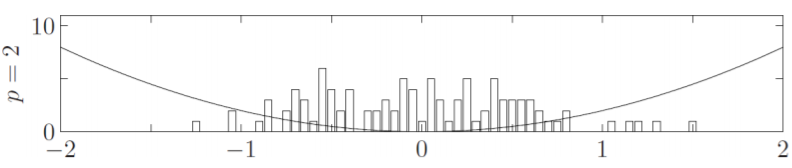
\includegraphics[width=\textwidth]{09/3_27}
        \caption{An histogram of the values taken by the weights shows how this regularizer tends to minimize an $x^2$ penalty for each weight, promoting \emph{shrinkage}. Notice how the quadratic penalty translates to having higher penalty on weights with larger norms, and viceversa.}	
    \end{figure}

    \item Lasso ($L_1$) regularization.
    \begin{figure}[H]
        \centering
        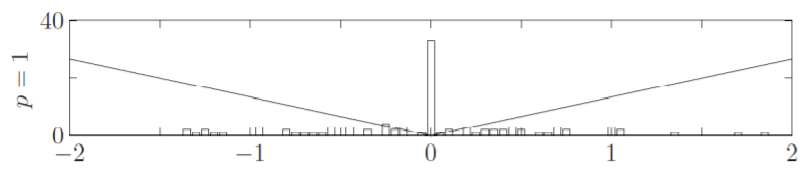
\includegraphics[width=\textwidth]{09/4_27}
        \caption{An histogram of the values taken by the weights shows how this regularizer tends to minimize an $x$ penalty for each weight, promoting \emph{sparsity} or \emph{weight selection}. Notice how every weight receives (proportionally) an equal penalty, and so most of them are at zero.}	
    \end{figure}

    \item Bounded $L_2$ norm at each layer $\norm{\mathbf{W}^{(\ell)}}_F \le c^{(\ell)}$, meaning that instead of just promoting small $L_2$ norm, it places an
    upperbound $c$ on the $L_2$ norm of the weights at a layer $\ell$. 
    
    \textbf{Note}. Formally we use the \emph{Frobenius} norm, which generalizes the $L_2$ norm to matrices, being the square root of the sum of all their entries squared.
    \begin{equation}
        \norm{M}_F = \sqrt{ \sum_i \sum_j |M_{i, j}|^2}.
    \end{equation}

\end{itemize}
After training, the $L_p$ magnitude of each weight reflects its importance in the final solution.\\


\paragraph{Sparsity}

Let's understand better how sparsity emerges with lasso regularization. We will use an example in $\mathbb{R}^2$, meaning we are considering a model with parameters $\vb*{\theta} = \mqty(\theta_1, \theta_2)^{\top}$, just to better visualize the situation. 

The loss function $\mathcal{L}: \mathbb{R}^2 \to \mathbb{R}$ can be visualized as isolines on the plane. Suppose $\vb*{\theta}_{opt}$ is where the optimum (minimum) of $\mathcal{L}$ is, which would be the result of a simple minimization of the loss function. Then with a minimization algorithm we would iteratively shift the weights from an initial point eventually to this point. Now suppose that we don't just want to minimize $\mathcal{L}$, but we are also enforcing a (hard) constraint: we want 
\begin{equation}
    \norm{\vb*{\theta}}_p \leq 1;
    \label{eq:9:1:constraint}
\end{equation}
then, in \cref{fig:09:1:penalties} we can see this with $p = 1$ ($L_1$ penalty) and $p = 2$ ($L_2$ penalty). 
\begin{figure}[H]
    \centering
    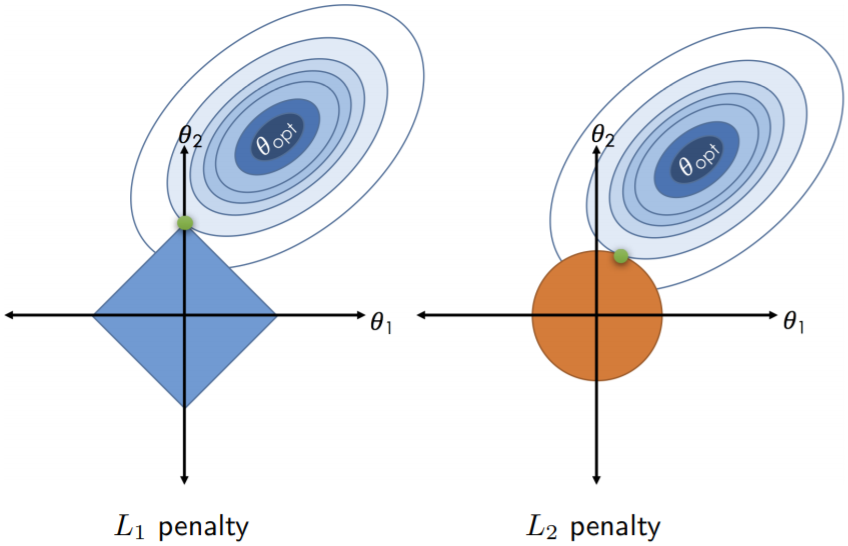
\includegraphics[width=.7\textwidth]{09/6_27}
    \caption{$L_1$ penalty vs $L_2$ penalty.}
    \label{fig:09:1:penalties}	
\end{figure}
Since the constraint is a hard constraint, the point $\vb*{\theta}$ is constrained to lie inside the locus of points satisfying \cref{eq:9:1:constraint}, and so to come as close as possible to the optimum, it will lie on the edge.
Notice that, using the $L_1$ penalty, the $\theta_1$ value goes to $0$; this is what we would call sparsity. This is not by chance; in fact, it can be formally shown that selecting a point at the corners of the $L_1$ ball is much more likely to happen than selecting a point at the intersection
between the sphere and an axis in the $L_2$ ball. For $L_1$ we will have very often a point on the corner (\emph{sparse solution}); for the $L_2$ we will have very often a point on the arc (\emph{non-sparse solution}).